% !TEX root = mythesis.tex

%==============================================================================
\chapter{Signal extraction and Background Estimation}
\label{sec:tZq}
%==============================================================================

\section{The \tZqsec production}
High energy proton-proton collisions at the LHC enable
multiple processes to occur simultaneously. Out of those processes, the process of 
interest for this analysis 
is the electroweak production of the \Ptop-quark and the 
\PZ-boson, referred to as the \tZq production. The LO $t$-channel Feynman diagrams are shown in \cref{fig:tZqfeyn} where
a \PZ-boson can be radiated from any one of the incoming or outgoing quarks (\cref{fig:tZqfeyna})
or from the exchanged \PW-boson (\cref{fig:tZqfeynb}). In addition to these
resonant contributions, there is also a small non-resonant contribution 
in the form of $tl^+l^-q$ (\cref{fig:tZqfeync}) which is also accounted for. The \Ptop-quark can be produced through
interactions such as $\Pup+\Pbottom \rightarrow \Pdown+\PZ+\Ptop$ or 
$\APup+\Pbottom \rightarrow \APdown+\PZ+\Ptop$ whereas \APtop-quark can be produced 
via charge conjugate processes. The NLO QCD
corrections for \tZq are small and therefore any possible deviations from the SM can be 
studied in the context of SM Effective Field Theory. 

\mynote[inline]{}{This will be useful when EFT section is written. Make sure the 
section is referenced}


\begin{figure}[htbp]
    \centering
    % \begin{subfigure}{0.35\figwidth}
    %   \centering
    %      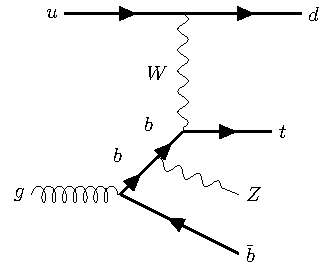
\includegraphics[width=\textwidth]{tZq_Zfromb.pdf}
    %      \caption{}
    %      \label{fig:tZqfeyna}
    % \end{subfigure}
    % \qquad
    \begin{subfigure}{0.35\figwidth}
      \centering
      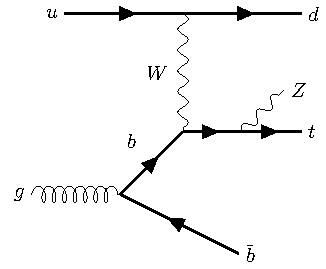
\includegraphics[width=\textwidth]{tZq_Zfromtop.pdf}
      \caption{}
      \label{fig:tZqfeyna}
    \end{subfigure}
    \begin{subfigure}{0.35\figwidth}
      \centering
      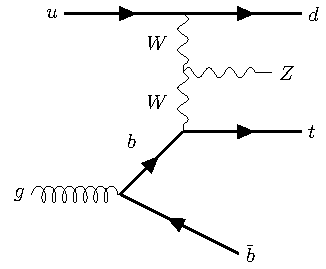
\includegraphics[width=\textwidth]{tZq_ZfromWW.pdf}
      \caption{}
      \label{fig:tZqfeynb}
    \end{subfigure}
  
  
  \medskip
  
  
  \begin{subfigure}{0.35\figwidth}
      \centering
      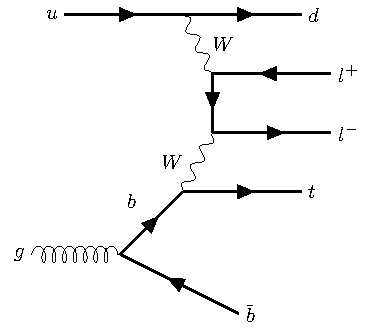
\includegraphics[width=\textwidth]{tZq_nonres.pdf}
      \caption{}
         \label{fig:tZqfeync}
    \end{subfigure}
    % \begin{subfigure}{0.35\figwidth}
    %   \centering
    %   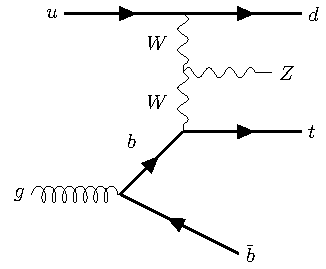
\includegraphics[width=\textwidth]{tZq_ZfromWW.pdf}
    %   \caption{}
    %      \label{fig:tZqfeyne}
    % \end{subfigure}
    % \begin{subfigure}{0.35\figwidth}
    %     \centering
    %     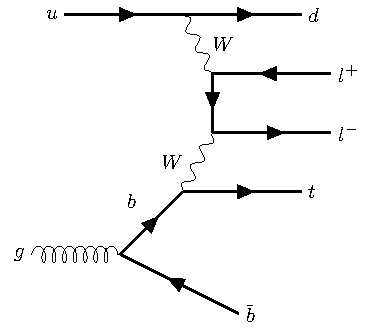
\includegraphics[width=\textwidth]{tZq_nonres.pdf}
    %     \caption{}
    %      \label{fig:tZqfeynf}
    %   \end{subfigure}
  
  \caption[Feynman diagrams at LO for the \tZq-production]{Feynman diagrams at 
  LO for the \tZq-production. The \PZ is radiated either from one of the
  quarks or from the exchanged W boson. }
  \label{fig:tZqfeyn}
  \end{figure}

The \tZq production probes the coupling of \Ptop and \PZ as well as the $\PW\PW\PZ$ coupling.
Hence, it allows the coupling
of two bosons and the coupling of a fermion to a boson to be studied in a single interaction. Moreover, 
it can provide a solid basis to study similar processes such as the $tHq$ process. 
The \mynote{expected cross-section}{check what cross-section we are quoting} of the \tZq production in the SM, calculated at NLO in QCD
for a dilepton mass more than $\qty{30}{\GeV}$, is $\qtypmerr{102}{5}{2}{\femto\barn}$. The
cross-section, measured by the ATLAS collaboration, is $\qtyerrs{97}{13}{7}{\femto\barn}$ which
is consistent with the SM expectation. 

In order to study this process, one has to note 
that the particles involved are quite heavy and therefore,
the only way to spot them is from their reconstructed decay products. 
Conventionally, the possible final states are divided into several \textit{channels}
based on certain combinations of leptons and jets. This analysis focuses on
the so-called trilepton channel as described below.

\section{The \tZqsec Trilepton Channel}
As the name suggests, the trilepton decay channel of the \tZq production 
contains final states with three charged leptons, as shown in \cref{fig:tZqtrilep}. The
\Ptop-quark decays almost exclusively into \Pbottom\PW and the corresponding \PW decays into a charged lepton and
an associated neutrino. The \PZ-boson decays into opposite sign same flavour lepton pairs and its probability 
is equal across the three lepton families (\Pelectron,\Pmuon,\Ptauon) due to 
lepton universality. This analysis includes \PZ decays resulting into electrons or muons 
(\Pelectron\APelectron or \Pmuon\APmuon). The \Ptauon-leptons are considered if they decay into lighter
leptons (i.e. \Pelectron or \Pmuon).

\mynote[inline]{}{Do we talk about other decay channels?}
The branching ratio of the trilepton channel is relatively small. However, it has a clean 
signature due to the three lepton requirement. In addition, three lepton final state is quite difficult
to mimic by background processes. This is the reason to choose this final state for studying \tZq process.
For this analysis, the trilepton final state is referred to as the signal.

\begin{figure}
  \centering
      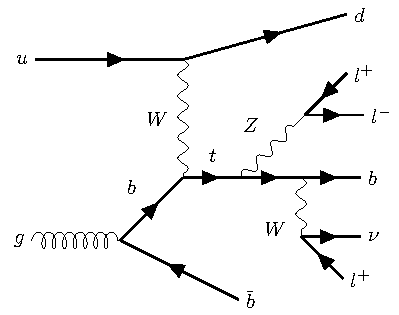
\includegraphics[width=0.45\textwidth]{tZq_Zfromtop_decay.pdf}
      \caption{The \tZq trilepton final state}
         \label{fig:tZqtrilep}
\end{figure}

\subsection{Event Selection}
The next task is to reconstruct this final state from the detector data or in other words, find
possible occurrences of this final state within the collision events. In order to achieve that,
certain requirements are defined in favour of the signal events. The collection of these requirements
is called event selection. For this analysis, the primary event selection is discussed below and
summarised in \cref{tab:selection:srcr}.

\begin{itemize}
  \item \textbf{Leptons}
    \begin{itemize}
      \item Exactly three leptons (\Pelectron or \Pmu), 
      \Ptau is considered if it decays into leptons. These leptons are 
      sorted by their \pT which is required to be at least 27,15 and 10 GeV, respectively.
      
      \item At least 1 Opposite Sign Same Flavour (OSSF) lepton pair with a minimum
      difference between its invariant mass ($m_{ll}$) and $m_Z$. This is to identify 
      which out of the selected leptons originate from \PZ.

      \item A cut on minimum accepted invariant mass, in order to suppress backgrounds 
      not containing a \PZ.

      \item A cut on the transverse mass of the \PW-boson is applied to account for the missing
      transverse energy. 
  \end{itemize}
  \item \textbf{Jets}
  \begin{itemize}
    \item Number of jets are required to be between 2 and 5, with \pT more than \qty{25}{GeV}
    and $|\eta|$ more than 4.5.
    \item Number of \Pbottom-jets are required to be 1 or 2, reconstructed at $85\%$ working 
    point with $|\eta|$ more than 2.5. Events with 2 jets, both \Pbottom-tagged are not considered.
  \end{itemize}


\end{itemize}

\begin{table}[!htbp]
    \footnotesize
    \caption{Event selection}
    \label{tab:selection:srcr}
    \renewcommand{\arraystretch}{1.3}
    \centering
    \begin{tabular}{lccc}
        \toprule
        Variable & \multicolumn{3}{c}{Preselection}\\
        \midrule
        $N_\ell~\left(\ell=e,\mu\right)$ & \multicolumn{3}{c}{$=3$}\\
        & \multicolumn{3}{c}{$\ge 1$ OSSF lepton pair}\\
        $\pT\left(\ell_1,\ell_2,\ell_3\right)$ & \multicolumn{3}{c}{$>$ 27,~15, \qty{10}{\GeV}}\\
        $\min(m_{\ell\ell})$ & \multicolumn{3}{c}{$>$ \qty{20}{\GeV}} \\
        $|m_{\ell\ell} - m_{Z}|$ & \multicolumn{3}{c}{$<$ \qty{10}{\GeV}} \\
        \mtw & \multicolumn{3}{c}{$>$ \qty{30}{\GeV}} \\
        $N_\text{jets}\left(\pT>25~\mathrm{GeV}\right)$ & \multicolumn{3}{c}{2-5} \\
        $N_{b-\text{jets}} @ 85\%$ & \multicolumn{3}{c}{1-2 (no $2j2b$)} \\
        % & SR & \CRttZ & \CRVV \\
        % $N_\text{jets}\left(\pT>25~\mathrm{GeV}\right)$ & 2-5 & $\ge 6$ & 2-5 \\
        % $N_{b-\text{jets}} @ 85\%$ & 1-2 (no $2j2b$) & $\ge 1$ & 0 \\
        \bottomrule
    \end{tabular}
    \end{table}


It is important to note here that these requirements are chosen to 
maximise the probability of selecting signal events
but in reality there are background processes that mimic the \tZq signature
and therefore, contaminate the selected signal events. 

\section{Background processes}

The background processes for \tZq process can be classified according to the number of prompt (or real)
leptons in the final state. A lepton is labelled prompt if it originates from either a \Ptau or a 
massive boson. On the other hand, non-prompt or fake leptons are objects misidentified as leptons.
The source of non-prompt leptons can be bottom and charm hadron decays, meson decays, 
photon conversions or light jets creating lepton-like signatures. Backgrounds involving only prompt leptons
are \diboson, \ttX, \ttH and \tWZ while backgrounds involving non-prompt leptons are \Ptop{}\APtop,
\PZ+jets and \tW.

\subsection*{Backgrounds involving prompt leptons}

In the \diboson process, two massive bosons are produced which can be \PZ{}\PZ, \PW{}\PW or \PW{}\PZ,
as shown in \cref{fig:VVfeyn}. As per \cref{fig:VVfeyna}, the leptonic decay of bosons result 
into three prompt leptons which can pass the signal event selection if additional jets are also found.
For the \PZ{}\PZ scenario, as shown in \cref{fig:VVfeynb}, one of the leptons needs to fail the 
requirement for a prompt lepton or is not reconstructed. Due to this strong resemblance of the 
\diboson signature with the signal, it is the dominant background in the \tZq production. 

\begin{figure}[htbp]
  \centering
  \begin{subfigure}{0.45\figwidth}
    \centering
    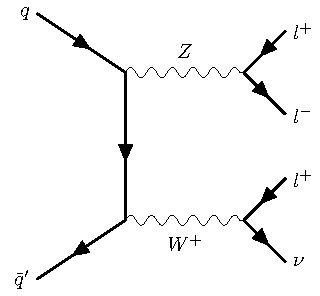
\includegraphics[width=\textwidth]{Feynman_WZ.pdf}
    \caption{}
    \label{fig:VVfeyna}
  \end{subfigure}
  \begin{subfigure}{0.45\figwidth}
    \centering
    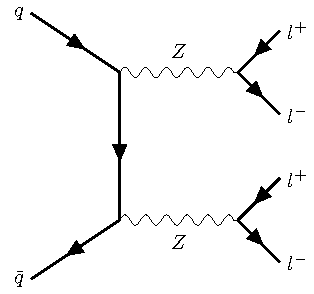
\includegraphics[width=\textwidth]{Feynman_ZZ.pdf}
    \caption{}
    \label{fig:VVfeynb}
  \end{subfigure}
  \caption[Feynman diagrams for \diboson backgrounds]{Feynman diagrams for the \diboson background}
  \label{fig:VVfeyn}
  \end{figure}

The \Ptop-quark pair production in association with a heavy boson (\PZ or \PW) can be an
important source of background. In particular, the \ttZ process, where the 
final state already includes a \PZ boson and a \Ptop quark, can produce a very 
similar signal-like signature. It is shown in \cref{fig:ttZ}. The \ttH contributes
less because of its small cross-section.

\begin{figure}
  \centering
      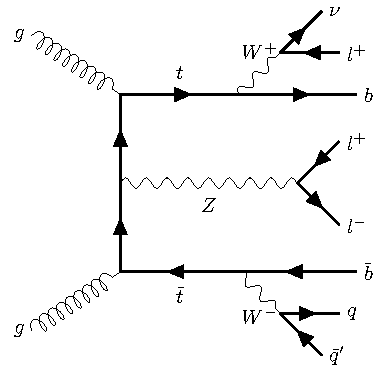
\includegraphics[width=0.45\textwidth]{Feynman_ttbarV.pdf}
      \caption{Feynman diagrams for the \ttZ background}
         \label{fig:ttZ}
\end{figure}

\subsection*{Backgrounds involving non-prompt leptons}

Backgrounds involving non-prompt or fake lepton are \Ptop-quark pair production 
and the production \PZ-boson with jets. 
As shown in \cref{fig:fakefeynb}, there are already two leptons
from the \PZ-boson. If the jets are light, they can be misidentified as leptons leading to 
a non-prompt lepton contribution.
In the \Ptop{}\APtop production, as shown in \cref{fig:fakefeynb}, if one of the \Pbottom-jet decays 
into a lepton, then it can satisfy the signal event selection.


\begin{figure}[htbp]
  \centering
  \begin{subfigure}{0.45\figwidth}
    \centering
    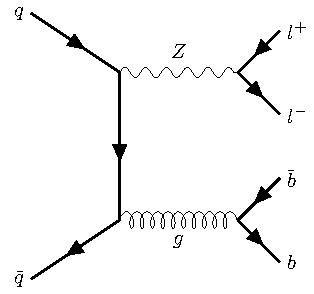
\includegraphics[width=\textwidth]{ZPlusJets_standalone.pdf}
    \caption{}
    \label{fig:fakefeyna}
  \end{subfigure}
  \begin{subfigure}{0.45\figwidth}
    \centering
    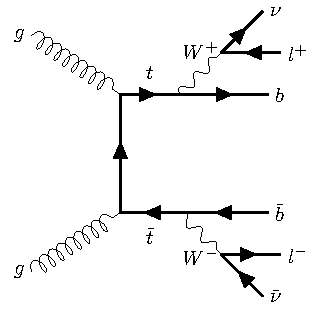
\includegraphics[width=\textwidth]{ttbar_standalone.pdf}
    \caption{}
    \label{fig:fakefeynb}
  \end{subfigure}
  \caption[Feynman diagrams for non-prompt lepton backgrounds]{Feynman diagrams for non-prompt lepton background}
  \label{fig:fakefeyn}
  \end{figure}

\section{Monte-Carlo (MC) simulations}

\mynote[inline]{}{can i put it after PDF? it is also a part of physic at hadron colliders!}

As already discussed before, proton-proton collisions are viewed as collisions between partons. This is 
not a simple process because multiple interactions can occur within the same event. With this complexity,
it becomes difficult to study the interaction of interest and more importantly the task of 
segregating signal from background becomes more complex. Here is where, Monte Carlo
generators come to the rescue. Monte Carlo generators are software that simulate collision events along with
detector effects and try to provide a detailed description of the possible final states. More precisely,
they use pseudo-random numbers to reproduce the quantum mechanical probabilities of different outcomes
of a collision event~\cite{mcgen}.  

The simulated data provided by these generators can be thought of as a "digital twin"
of the actual observed data. It can be used to predict any experimental observable or a combination of observables.
The MC chain is a step-by-step process that begins with identifying the hard interaction and 
continues until the final state is achieved. At each stage, the structure of the underlying event 
evolves. The steps are briefly summarised below:

\begin{itemize}
  \item \textbf{Hard process}: In this step the hard process, defined as the process with highest
  momentum transfer, is determined using matrix element calculation combined with the input Parton
  Distribution Functions. If a resonance is produced in a hard process, such as the \Ptop or \PZ and it
  shortly decays, then its decay process is also considered within the hard process. 

  \item \textbf{Parton Shower (PS)}: The colliding partons are responsible for emissions that give rise
  to more partons and subsequently more interactions. The emissions associated with the incoming partons
  is called Initial-State Radiation (ISR) while the emissions associated with outgoing partons is called
  Final-State Radiation (FSR). These emissions and their respective interactions are modelled with
  Parton Shower algorithms. The incorporation of PS into the matrix element paints a more accurate picture
  of the collision process.

  \item \textbf{Multiple-processes}: Until now, only one of the partons from the original hadron is 
  considered but in reality, other partons from the same hadron also interact. Their interactions are
  termed as multiple-processes and they are calculated at this step of the MC simulation chain.
  
  \item \textbf{Hadronisation and decay}: The outgoing partons, with sufficient energy, can produce 
  new hadrons due to QCD colour confinement (hadronisation). If these hadrons are unstable, they can also
  decay into lighter particles. The MC chain also includes these calculations.
\end{itemize}

Finally, detector simulation is applied, after which the simulated data is ready for comparison with the 
detector data.
% After all the MC events are generated, the GEANT4 software toolkit [12] is used to propagate
% the particles through the detector and to simulate their interactions with the detector material.
Among the various available MC generators, \textsc{Herwig}~\cite{Bellm2016} and 
\textsc{Pythia}~\cite{SJOSTRAND2008852} are two of the most commonly used ones.

\mynote[inline]{}{explain the different weights}

\section{Data and simulated samples}
This analysis uses collision data collected by the ATLAS detector during 2015 to 2018 (Run-2 of the LHC) at a center of
mass energy of \qty{13}{\GeV}. The total integrated luminosity is of \lumi.

The ATLAS MC samples for analysis of the Run-2 dataset are divided into three subsets: 
\texttt{mc16a} generated with 2015 an 2016 pileup conditions, \texttt{mc16d} generated with 
2017 pileup conditions and \texttt{mc16e} that includes pileup conditions of 2018 data. 

\subsection{Signal sample}
The \tZq signal sample is simulated using \textsc{MadGraph5\_aMC@NLO} 2.9.5 generated at next-to-leading
order (NLO) with \textsc{NNPDF3.0NLO} parton distribution function. In general, the models used for
PS and hadronisation contain several free parameters which must be optimised to generate a reasonable
description of data. The optimisation is termed as tuning and the resulting sets of parameters are called
tune sets. For the signal sample, \textsc{Pythia} 8.245 is used for Parton Shower and
hadronisation along with A14 (ATLAS 24~\cite{ATL-PHYS-PUB-2014-021}) tune set and the \textsc{NNPDF2.3LO} PDF set.
The \Ptop-quark is decayed at LO using \textsc{MADSPIN}.
\mynote[inline]{}{UPDATE THIS AFTER NEW SAMPLE and add info about scales}

\subsection{Background samples}
For the background processes, different versions of \textsc{MadGraph5\_aMC@NLO}~\cite{Alwall:2014hca}, 
\textsc{Sherpa}~\cite{TGleisberg_2009} or \textsc{Powheg}~\cite{Banfi:2023mhz} generators are used to
calculate the matrix element and cross-sections combined with the \textsc{NNPDFx.xNLO} PDF set.
The PS and hadronisation is modeled with \textsc{Pythia} for the nominal background samples
and \textsc{Herwig} for the alternate sample generation. The alternate samples are required
for the theoretical uncertainties as described in SECTION. The specific versions
used for different backgrounds is summarised in \cref{tab:bkgmc}.

\mynote[inline]{}{Add the detailed DSIDs and everything in the appendix and refer here}

\begin{table}[htbp]
  \tablesetup
  \centering
  \caption{Background sample details} 
  \begin{tabular}{ l | l | l | l | l }
  \toprule
  Background & Generator &  Parton Shower &  PDF & Type of Sample \\
  \midrule
  \ttZ & \textsc{MadGraph5\_aMC@NLO} 2.8.1 & \textsc{Pythia} 8.244 & \textsc{NNPDF3.0NLO} & Nominal \\
  & & & \textsc{NNPDF2.3LO} & \\
  \ttZ & \textsc{MadGraph5\_aMC@NLO} 2.8.1 & \textsc{Herwig} 7.2.1 & \textsc{NNPDF3.0NLO} & Alternate \\
  & & & \textsc{NNPDF2.3LO} & \\
  \tWZ & \textsc{MadGraph5\_aMC@NLO} 2.X.X & \textsc{Pythia} 8.235 & \textsc{NNPDF3.0NLO} & Nominal \\
  \Diboson & \textsc{Sherpa} 2.2.12 & \textsc{Sherpa} \textsc{MEPS@NLO} & \textsc{NNPDF3.0NNLO} & Nominal \\
  \Triboson & \textsc{Sherpa} 2.2.2 & \textsc{Sherpa} \textsc{MEPS@NLO} & \textsc{NNPDF3.0NNLO} & Nominal \\
  \ttbar & \textsc{Powheg Box v2} & \textsc{Pythia} 8.230 & \textsc{NNPDF3.0NLO} & Nominal \\
  & & & \textsc{NNPDF2.3LO} & \\
  \ttbar & \textsc{Herwig} 7.2.1 & \textsc{Pythia} 8.230 & \textsc{NNPDF3.0NLO} & Alternate \\
  \tW & \textsc{Powheg Box v2} & \textsc{Pythia} 8.230 & \textsc{NNPDF3.0NLO} & Nominal \\
  & & & \textsc{NNPDF2.3LO} & \\
  \Zjets & \textsc{Sherpa} 2.2.11 & \textsc{Sherpa} \textsc{MEPS@NLO} & \textsc{NNPDF3.0NNLO} & Nominal \\
  \ttW & \textsc{Sherpa} 2.2.10 & \textsc{Sherpa} \textsc{MEPS@NLO} & & Nominal \\
  \ttH & \textsc{Powheg Box v2} & \textsc{Pythia} 8.230 & \textsc{NNPDF3.0NLO} & Nominal \\
  & & & \textsc{NNPDF2.3LO} & \\
  \ttt & \textsc{MadGraph5\_aMC@NLO} 2.2.2 & \textsc{Pythia} 8.186 & \textsc{NNPDF2.3LO} & Nominal \\
  \tttt & \textsc{MadGraph5\_aMC@NLO} 2.3.3 & \textsc{Pythia} 8.230 & \textsc{NNPDF3.1LO} & Nominal \\
  \tttt & \textsc{MadGraph5\_aMC@NLO} 2.3.3 & \textsc{Herwig} 7.0.4 & \textsc{NNPDF3.1LO} & Alternate \\
  \bottomrule
  \end{tabular}
  \label{tab:bkgmc}
  \end{table}

\section{Systematic Uncertainties}
One of the key advantages of using simulated data is their ability to predict how the observed data may appear. 
However, it is crucial to assess how dependable both the simulated and the measured data are, which
is quantified through uncertainties. The proper inclusion of uncertainties is an important part of any analysis.

Uncertainties can be divided into two sections: statistical and systematic. Simply put, statistical uncertainties are
related to the statistics of the data whereas systematic uncertainties are complex uncertainties 
that are not directly from the statistics of the data. For instance, the length of an object is measured with a 
ruler and is found to be $10 \pm 0.5$ cm. Here the statistical uncertainty is $0.5$ cm. In addition,
there is a systematic uncertainty which can originate from the calibration of the ruler. 

In high energy physics, sources of systematic uncertainties are calibrations of scales, efficiencies of 
particle identifications and reconstructions, choice of MC generators, etc. These sources of systematic
uncertainties are categorised into: instrumental and theoretical uncertainties as described
in \cref{sec:systdescribe} and \cref{sec:systdescribe2}, respectively. 

\subsection{Instrumental or detector uncertainties}
\label{sec:systdescribe}

\begin{itemize}
  \item \textbf{Luminosity}: The integrated luminosity is \lumi and the uncertainty in its calculation
  is $0.83\%$

  \item \textbf{Pileup reweighting}: MC generators make use of scale factors to account for differences in 
  pileup distributions between data and simulations. There is an uncertainty associated with these 
  scale factors. It is evaluated by changing the nominal pileup value to a lower and a higher value,
  then the effect of these changes is calculated to obtain the up and down uncertainty.

  \item \textbf{Jet Energy Scale (JES)}: After the jets are reconstructed, their energies need to be 
  adjusted so that it reflects the energy of the colliding particles. The calibration is done by 
  comparing the reconstructed jets with the true jets which are simulated jets of stable particles 
  without detector effects. Uncertainties originating from the calibration process are categorised 
  as JES uncertainties~\cite{Barillari2012}.

  \item \textbf{Jet Energy Resolution (JER)}: JER is the detector's ability to distinguish two jets 
  with similar total energy. The uncertainty associated with the differences in JER in case of data and 
  simulation is called JER uncertainty. 

  \item \textbf{Lepton reconstruction}: Scale factors are applied to correct differences between data and
  simulation in case of lepton identification, isolation and trigger efficiencies. The uncertainties
  associated with these scale factors belong to the lepton reconstruction category of systematics.  

\end{itemize}

\subsection{Theoretical uncertainties}
This category involves uncertainties originating from the various models used in the MC simulation 
chain, and therefore, also called modeling uncertainties or modeling systematics. 
  
\begin{itemize}
  
  \item \textbf{A14}: The uncertainty associated with the A14 tune set is determined by comparing the nominal sample with 
  two alternate samples, both simulated using the same settings as the nominal sample but incorporating 
  the up and down variations of the A14 tune set. This variation is related to the strong 
  coupling constant $\alpha_s$. This uncertainty is considered for \tZq and \ttZ processes. 

  \item \textbf{Scale}: The scale uncertainty is calculated by using a 3-point variation. The parameters
  $\mu_R$ and $\mu_F$, related to $H_T/6$, are varied between 0.5, 1 and 2. This uncertainty is considered 
  for \tZq and \ttZ processes. 
  \mynote[inline]{}{What is mur muf and rephrase this}

  \item \textbf{Shower and PDF}: The showering uncertainty is calculated by comparing the nominal sample (modeled using \textsc{Pythia})
  and the alternate sample (modeled using \textsc{Herwig}). Moreover, uncertainty associated 
  with the PDF is also considered. This uncertainty is considered for \tZq and \ttZ processes. 

  \item \textbf{\tWZ modeling} This uncertainty accounts for the interference between \ttZ and \tWZ
  processes. The non-resonant \tWZ production can feature a resonant $\APtop$ in the intermediate state,
  leading to overlap with the \ttZ production. This interference is navigated using various techniques 
  called diagram removal (DR) and diagram subtraction (DS). Two \tWZ samples were generated, one with 
  DR1 and another with DR2 and the difference is taken to be the \tWZ modeling uncertainty. 

  \item \textbf{\diboson }
\end{itemize}
\label{sec:systdescribe2}


\section{Artificial Neural Networks}
A neural network is a computation tool developed to function in a way similar to the human mind. It is 
widely used in high energy physics for data analysis. The structure of a neural network (NN) is made 
up of neurons or \textit{nodes}. Their function is to examine unknown systems and identifying 
interesting features, just like the job of neurons in human mind. Generally, these nodes are arranged 
in three different layers: the input layer, the hidden layer and the output layer. A list of variables 
is given as input to the nodes of the input layer. Processing takes place through the subsequent 
layers and at the end, the output layer returns the conclusions derived by the network. Connections 
between nodes of different layers are referred to as the \textit{synapses}. Each connection between 
nodes of two consecutive layers, has a weight associated to it. 
% Figure~\ref{fig: 4.8} shows a diagram of a neural network. 

% \begin{figure}[htbp]
%   \centering
%     \includegraphics[width=0.7\figwidth]{nn.png}
%   \caption[Neural Network]{Diagram of a neural network including the input, hidden and output layers~\cite{NN}.}
%   \label{fig: 4.8}
% \end{figure}

The input received by each node is the sum of weighted output of all nodes of the previous layer. 
As given in Equation~\ref{eqn:4.2}, $y_j$ is the input to node $j$, $w_{ij}$ is the weight from the 
$i$-th node and $x_i$ is that node's output. The term $w_{0j}$ is called bias. 

\begin{equation}
    y_j = \Sigma_{i=1}^{n} w_{ij}x_i + w_{0j} 
    \label{eqn:4.2}
\end{equation}


The output of a node is defined by an \textit{activation} function. Common choice of an activation 
function is the sigmoid function. It provides output between 0 and 1. A feature that makes a NN special
is its capability to \textit{learn} from examples with known inputs and outputs. This is referred to 
as \textit{training} a neural network. The purpose of training is to find appropriate weights. 
In supervised training, inputs and outputs are provided to a NN. It processes input and then compares 
the resultant output with the desired output. Comparison is done by calculating 
a \textit{loss function}. It is a way to determine how well is the network trained. For better
performance of a network the loss function should be minimised. In order to do that, errors of the 
resultant output are propagated back in a model and the initial weights are readjusted so that 
output is closer to the desired output. This is how a network learns. A dataset flows inside a 
network several times and each time weights are refined until a minimum value of the loss function 
is obtained.
